\documentclass{article}


\usepackage{amsmath}
\usepackage{amsthm}
\usepackage{amssymb,latexsym,color}
\usepackage{mdwlist}
\usepackage{fullpage}
\usepackage{charter}

\usepackage{url}

\usepackage{algorithm}
\usepackage[noend]{algpseudocode}

\usepackage{fullpage}
\usepackage{marvosym}
%\usepackage[techreport]{systems-cover}

\usepackage{graphicx}
\graphicspath{ {Figures/} }
\usepackage{subcaption}
%\captionsetup[subfigure]{justification=justified,singlelinecheck=false}

\newcommand{\R}{\mathsf{R}}
\newcommand{\sgn}[1]{\mbox{sgn}(#1)}
\renewcommand{\vec}[1]{\mathbf{#1}}
\newcommand{\poly}{\mathrm{poly}}

\def\a{{\bf a}}
\def\g{{\bf g}}
\def\x{{\bf x}}
\def\y{{\bf y}}
\def\w{{\bf w}}
\def\E{\mathbb{E}}
\def\rrow{r_\mathrm{row}}

\newcommand{\err}{\ensuremath{\mathrm{err}}}
\newcommand{\setX}{\Omega}
\newcommand{\setI}{\mathcal{I}}
\newcommand{\OPT}{\ensuremath{\mathrm{OPT}}}
\newcommand{\setF}{\mathcal{F}}
\newcommand{\setJ}{\mathcal{J}}


\DeclareMathOperator*{\argmin}{argmin}

\newtheorem{lemma}{Lemma}
\newtheorem{theorem}{Theorem}
\newtheorem{claim}{Claim}
\newtheorem{corollary}{Corollary}
\newtheorem{prop}{Proposition}
\newtheorem{definition}{Definition}

\newcommand{\todo}[1]{\noindent \textbf{[TODO:] #1 } }
\usepackage{mathtools}
\DeclarePairedDelimiter\floor{\lfloor}{\rfloor}
\DeclarePairedDelimiter\ceil{\lceil}{\rceil}
%\newcommand{\E}{\mathbb{E}}

%\input{settings-custom.tex} 
%\linespread{0.95}
%\includepackage{algorithm}




\date{}


\title{\small \bf
Supplementary Material
}

\begin{document}
\maketitle

\section{Preliminaries}

\subsection{Computational Model}

We consider a computational model illustrated in
Figure~\ref{fig:model}.  
In this context, SGD is often bounded by the bandwidth
of data movements cross these components. 
In particular, we consider the convergence properties of the algorithm when a lossy compression scheme is applied to the data (samples), 
gradient, and model, for the purpose of reducing the communication cost of the algorithm. 
It is interesting to consider how lossy compression impacts the update step in SGD. Let $Q( \vec{v} )$ denote the compression scheme applied to a vector $\vec{v}$. 

\begin{itemize}
    \item \textbf{Original iteration}: $$\x_{t + 1} \leftarrow \x_t - \gamma \g_k (\x_t, \vec{a}_t).$$
    \item \textbf{Compressed gradient}: $$\x_{t + 1} \leftarrow \x_t - \gamma Q( \g_k (\x_t, \vec{a}_t) ).$$
    \item \textbf{Compressed model}: $$\x_{t + 1} \leftarrow \x_t - \gamma \g_k (Q(\x_t), \vec{a}_t).$$
    \item \textbf{Compressed sample}: $$\x_{t + 1} \leftarrow \x_t - \gamma \g_k (\x_t, Q(\vec{a}_t)).$$
    \item \textbf{End-to-end compression}: $$\x_{t + 1} \leftarrow \x_t - \gamma Q(\g_k (Q(\x_t), Q(\vec{a}_t))).$$
\end{itemize}










\begin{figure*}[t]
\centering   
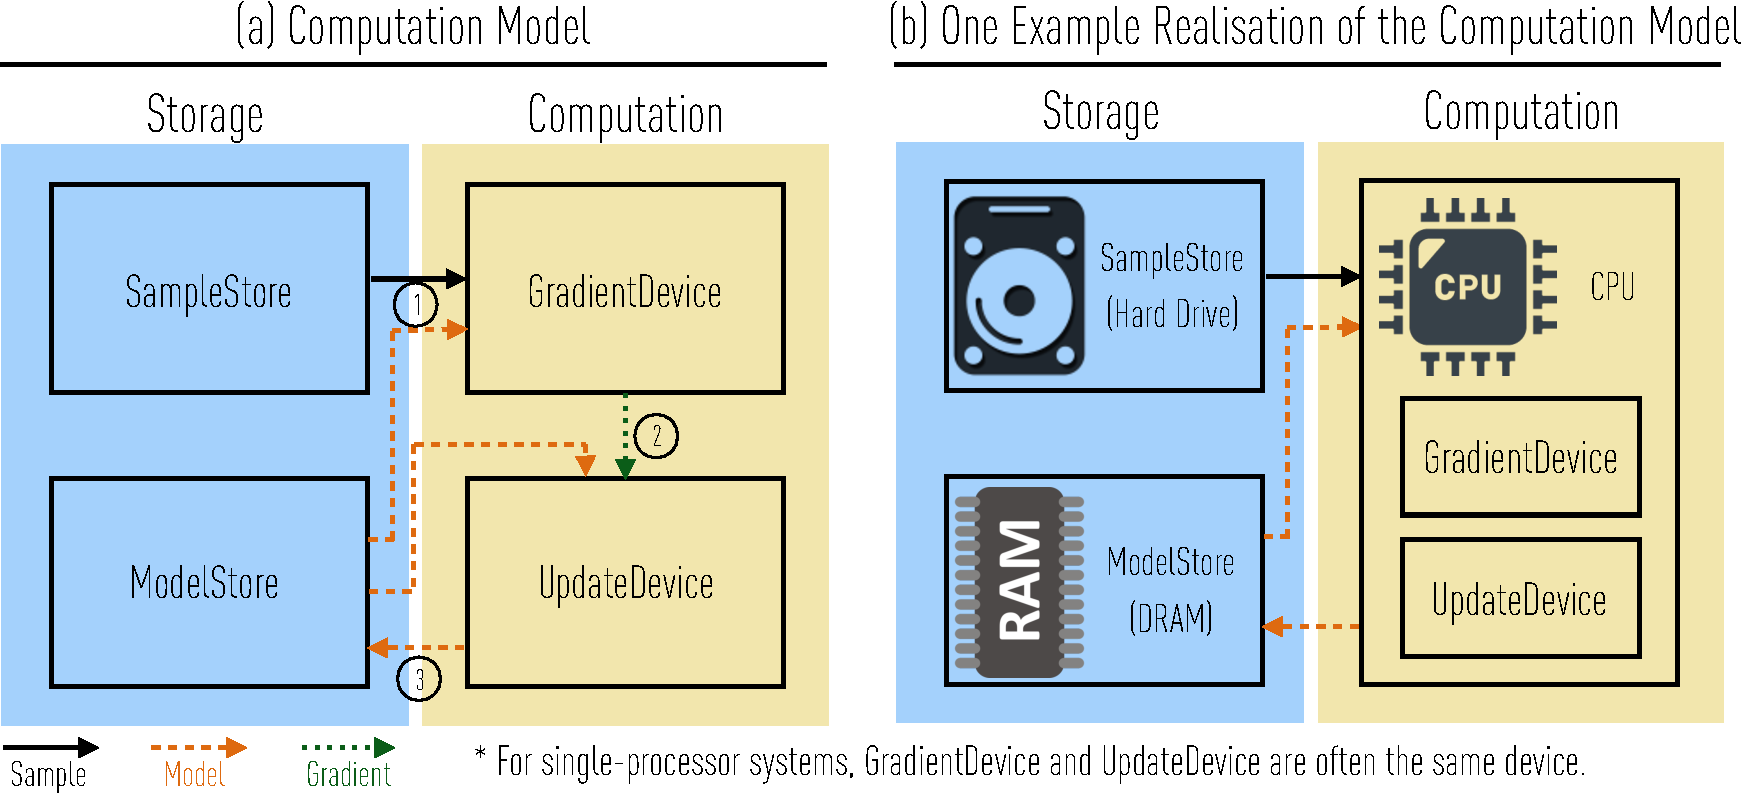
\includegraphics[scale=0.4]{compmodel-pdfcrop}
\caption{(a) A Schematic Representation of the Computation Model and (b) An Example Realisation
of the Computation Model. Three types of
data, namely (1) sample, (2) model, and (3)
gradient, moves in the system in three
steps as illustrated in (a). Given
different parameters of the computation model,
such as computational power and memory bandwidth, the system bottleneck may
vary. For example, in 
realisation (b) having a hard drive, DRAM, and a
modern CPU, it is likely that the  bottleneck when training 
a dense generalized linear model is the
memory bandwidth between SampleStore
and GradientDevice.}
\label{fig:model}
\end{figure*}






%\begin{figure}[h]
%\centering
%   
%    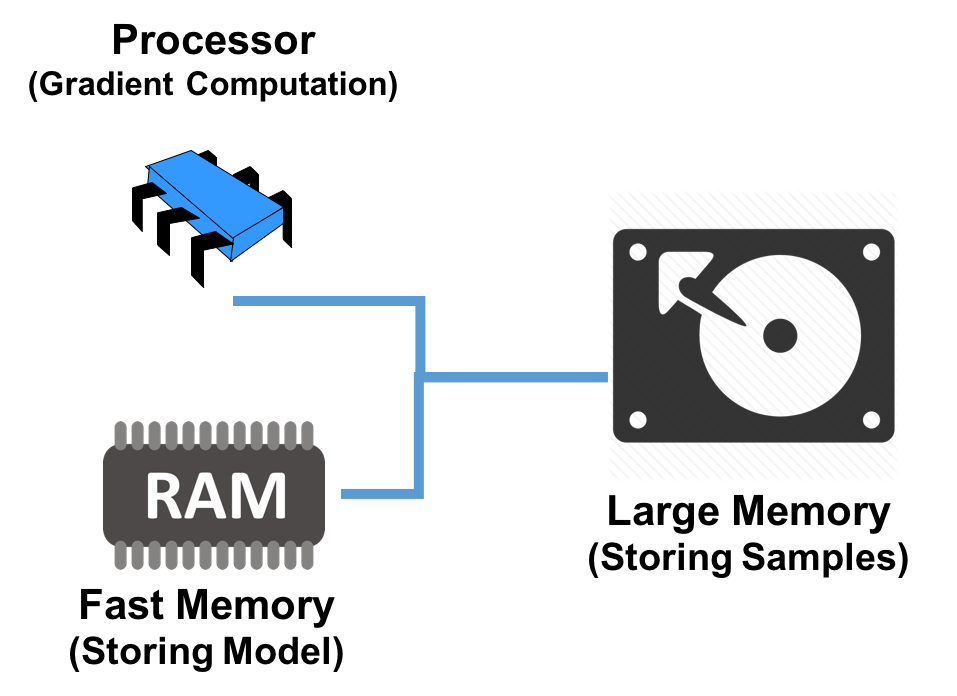
\includegraphics[scale=0.4]{schematic}
%    
%\caption{Simple Schematic of the %Computational Model}
%\label{fig:model}
%\end{figure}

\subsection{Guarantees for SGD}
In this paper we consider SGD, a general family of stochastic first order methods for finding the minima of convex (and non-convex) functions.
Due to its generality and usefulness, there is a vast literature on SGD in a variety of settings, with different guarantees in all of these settings.
Our techniques apply fairly generally in a black box fashion to many of these settings, and so for simplicity we will restrict our attention to a fairly basic setting.
For a more comprehensive treatment, see \cite{Bubeck15}.

Throughout the paper, we will assume the following setting in our theoretical analysis.
Let $\mathcal{X} \subseteq \R^n$ be a known convex set, and let $f: \mathcal{X} \to \R$ be differentiable, convex, and unknown.
We will assume the following, standard smoothness condition on $f$:
\begin{definition}[Smoothness]
Let $f: \R^n \to \R$ be differentiable and convex.
We say that it is $L$-smooth if for all $\x, \y \in \R^n$, we have
\[0 \leq f(\x) - f(\y) - \nabla f(\y)^T (\x - \y) \leq \frac{L}{2} \| \x - \y \|_2^2 \; .\]
\end{definition}

We assume repeated access to stochastic gradients, which on (possibly random) input $\vec{x}$, outputs a direction which is in expectation the correct direction to move in.
Formally:
\begin{definition}
Fix $f: \mathcal{X} \to \R$.
A \emph{stochastic gradient} for $f$ with bias bound $\beta$ is a random function $g (\x)$ so that $\E [g (\x) ] = G( \x)$, where $\| G(\x) - \nabla f(\x) \|_2 \leq \beta$ for all $x \in \mathcal{X}$.
%A \emph{stochastic oracle} for $f$ is an oracle which on (possibly random) input $\vec{x}$, outputs a stochastic gradient for $f$ at $\vec{x}$.
We say the stochastic gradient has second moment at most $B$ if $\E [\| g \|_2^2] \leq B$ for all $\x \in \mathcal{X}$.
We say it has variance at most $\sigma^2$ if $\E [\| g (\x) - \nabla f(\x) \|_2^2] \leq \sigma^2$ for all $\x \in \mathcal{X}$. 
\end{definition}

For simplicity, if $\beta = 0$ we will simply refer to such a random function as a stochastic gradient.
Under these conditions, the following convergence rate for SGD is well-known:

\begin{theorem}[e.g. \cite{2014arXiv1405.4980B}, Theorem 6.3]
\label{thm:sgd}
Let $\mathcal{X} \subseteq \R^n$ be convex, and let $f: \mathcal{X} \to \R$ be an unknown, convex, and $L$-smooth.
Let $\x_0 \in \mathcal{X}$ be given, and let $R^2 = \sup_{\x \in \mathcal{X}} \| \x - \x_0 \|_2^2$.
Suppose we run projected SGD on $f$ with access to independent stochastic gradients with bias bound $\beta$ and variance bound $\sigma^2$ for $T$ steps, with step size $\eta_t = 1 / ( L + \gamma^{-1})$, where $\gamma = \frac{R}{\sigma} \sqrt{\frac{2}{T}}$, and
\begin{equation}
\label{eq:sgd-conv}
T = O \left( R^2 \cdot \max \left( \frac{2 \sigma^2}{\epsilon^2} , \frac{L}{\epsilon} \right) \right) \; .
\end{equation}
Then $\E \left[ f \left( \frac{1}{T} \sum_{t = 0}^T \x_t \right) \right] - \min_{\x \in \mathcal{X}} f(\x) \leq \epsilon + R \beta + \frac{\eta}{2} \beta^2$.
\end{theorem} 

In particular, note that the complexity the SGD method is mainly controlled by the variance bound $\sigma^2$ we may obtain. If $\sigma = 0$, the complexity is consistent with the stochastic gradient.


\subsection{Randomized Quantization}

In this section, we give a procedure to quantize a vector or real values randomly, reducing its information content. We will denote this quantization function by $Q(\vec{v},s)$, where $s\geq 1$ is the tuning parameter. 
Let $M(\vec{v}): \R^n \rightarrow \R^n$ be a positive scaling function such that, for $\vec{v}\in \R^n$, $\frac{\vec{v}_i}{M_i(\vec{v})} \in [-1, 1]$, where $M_i(\vec{v})$ denotes the $i$th element of $M(\vec{v})$.
For $\vec{v} \neq \vec{0}$ we define

\begin{equation}
Q_i(\vec{v},s) = M_i(\vec{v}) \cdot \sgn{\vec{v}_i} \cdot \mu_i(\vec{v},s) \; , \label{equ:quant2}
\end{equation}
where $\mu_i(\vec{v},s)$'s are independent random variables defined as follows. 
Let $0 \leq \ell < s$ be an integer such that $|\vec{v}_i|/M_i(\vec{v}) \in [ \ell / s, (\ell + 1) / s ]$, that is, $\ell = \lfloor s |\vec{v}_i|/\| \vec{v} \| \rfloor$. 
Here, $p(x,s) = x s - \ell$ for any $x \in [0,1]$.
Then 
\[
\mu_i(\vec{v},s) = \left\{ \begin{array}{ll}
         \ell / s & \mbox{with probability $1 - p\left(\frac{|\vec{v}_i|}{M(\vec{v})},s\right)$};\\
         (\ell + 1) / s & \mbox{otherwise}. \end{array} \right.
\]
If $\vec{v} = \vec{0}$, then we define $Q(\vec{v},s) = \vec{0}$.
For any such choice of $M_i$, we have the following properties, which generalize Lemma 3.4 in~\cite{QSGD}.
The proofs follow immediately from those in \cite{QSGD}, and so we omit them for conciseness.
\begin{lemma}
\label{lem:quant-facts}
 For any $\vec{v} \in \R^n$, we have that 
 \begin{itemize} 
 \item (Sparsity) $\E[ \|Q(\vec{v}, s)\|_0]\leq
 s^2 +\sqrt{n}$ , 
 \item (Unbiasedness) $\E [Q (\vec{v},s)] = \vec{v}$ , and
 \item (Second Moment Bound) 
$\E [\| Q (\vec{v},s) \|_2^2] \leq r M^2$, where $M = \max_i M_i (\vec{v})$, and 
\[
r = r(s) = \left( 1 + \frac{1}{s^2} \sum_{i = 1}^n p\left( \frac{|\vec{v}_i|}{M_i },s \right) \right) \; .
\]
 \end{itemize}
\end{lemma}


We now discuss different choices of the scaling function $M_i(\vec{v})$.

\paragraph*{``Row Scaling''}

One obvious choice that was suggested in \cite{QSGD} is to have $M_i(\vec{v}) = \| \vec{v} \|_2$, in this way, we
always have $\frac{\vec{v}_i}{M_i(\vec{v})} \in [-1, 1]$ and all $M_i(\vec{v})$ are the same
such that we can store them only once.
When the 
In the following, we will often use the version with $s = 1$, which is as follows. 
\begin{equation}
\label{equ:quant1}
Q_i(\vec{v}) = \| \vec{v} \|_2 \cdot \sgn{\vec{v}_i} \cdot \mu_i (\vec{v}) \; ,
\end{equation}
where $\mu_i(\vec{v})$'s are independent random variables such that $\mu_i(\vec{v}) = 1$ with probability $|\vec{v}_i| / \| \vec{v} \|_2$, and $\mu_i(\vec{v}) = 0$, otherwise. If $\vec{v} = \vec{0}$, we define $Q(\vec{v}) = \vec{0}$. 
%
Obviously, if
all vectors $\vec{v}$ are scaled to have unit $\ell_2$ norms, $M(\vec{v}) \equiv 1$
and therefore, we can also omit this term.
Moreover, it was shown in \cite{QSGD} that for this choice of $M_i$, the function $r$ can be upper bounded by
\[
r(s) \leq \rrow (s) = 1 + \min\left( \frac{n}{s^2}, \frac{\sqrt{n}}{s} \right) \; .
\]

\paragraph*{``Column Scaling''}
Let $\vec{v} \in \R^n$ be a sample and $V \subset \R^n$ be the set of sample vectors. 
%Another choice, especially when $\vec{v} \in \R^n$ is an input sample and 
We can obtain the upper and lower bound for each feature, that is,
%$the {\em constant} for each $\vec{v}_i$ such that Another choice, especially when $\vec{v} \in \R^n$ is an input sample and we know the {\em constant} for each $\vec{v}_i$ such that 
\[
\text{min}_i \le \vec{v}_i \le  \text{max}_i\quad \vec{v} \in V
\]
is to have $M_i(\vec{v}) = \max(|\text{min}_i|, |\text{max}_i|)$.
When the input samples are stored as a matrix in which each row corresponds
two a vector $\vec{v}$, getting $\min_i$ and $\max_i$
is just to getting
the $\min$ and $\max$ for each column (feature).
Using this scheme, all input samples can share the same
$M_i(\vec{v})$ and thus can be easily stored in cache when all
input samples are accessed sequentially (like in SGD).


\paragraph*{Choice between Row Scaling and Column Scaling}

In this working paper, we make the following choices regarding row scaling
and column scaling and leave the more general treatment to future work.
For all input samples, we always use column scaling because it is easy
to calculate $M_i$ which does not change during training. For all gradients
and models, we use row scaling because the range of values is more dynamic.

\section{Compressing the Samples for Linear Regression}

In this section, we will describe lossy compression schemes for data samples, so that when we apply SGD to solve linear regression on these compressed data points, it still provably converges.
Throughout this section, the setting will be as follows.
We have labeled data points $(\a_1, b_1), (\a_2, b_2), \ldots, (\a_K, b_K) \in \R^n \times \R$, and our goal is to minimize the function
\[
f(\x) = \frac{1}{K} \sum_{k = 1}^K \| \a_k^\top \x + b_k \|_2^2 \; ,
\]
i.e., minimize the empirical least squares loss.
The basic (unquantized) SGD scheme which solves this problem is the following: at step $\x_k$, our gradient estimator is $\g'_k = \a_{\pi(k)} (\a_{\pi(k)}^\top \x + b_{\pi(k)})$, where $\pi(k)$ is a uniformly random integer from $1$ to $m$.
In a slight abuse of notation we let $\a_k = \a_{\pi(k)}$ for the rest of the section.
Then it is not hard to see that $\E [\g'_k] = \nabla f(\x_k)$, and so this is indeed a stochastic gradient.

The rest of the section is now devoted to devising quantization schemes for $\g'_k$ when given access only to $\a_k$ and $b_k$, namely, given access only to the data points.

\subsection{Naive Random Quantization is Biased}

As a first exercise, we look at what happens when we work with the data directly in quantized form in the context of linear regression. 
The gradient becomes
\[
\g_k := Q(\a_k, s ) Q(\a_k, s)^\top \x + Q(\a_k, s) b_k.
\]
It is not hard to see that the expected value of this is in fact: 
\[
\E[\g_k] := \a_k \a_k^\top \x + \a_k b_k + D_{s, \a} \x, 
\]
where $D_{s, \a}$ is a diagonal matrix and its $i$th diagonal element is 
\[
%D_{s, \a} = 
\E[ Q(\a_i, s)^2 ] - \a_i^2.
\]

Since $D_{s, \a}$ is non-zero, we obtain a \emph{biased} estimator of the gradient, so the iteration is unlikely to converge. 
In fact, it is easy to see that in instances where the minimizer $\x$ is large and gradients become small, we will simply diverge. 
Fortunately, however, this issue can be easily fixed. 

\subsection{Double Sampling}

\paragraph{Algorithm}
Instead of the naive estimate, our algorithm is as follows.
We generate two independent
random quantizations $Q_1$
and $Q_2$ and revise the gradient as follows:

%\[
%\g_k := \frac{1}{2}\left(Q_1(\a_k ) Q_2(\a_k)^\top \x + Q_2(\a_k) b_k + Q_2(\a_k ) %Q_1(\a_k)^\top \x + Q_1(\a_k) b_k\right).
%\]

%\[
%\g_k := Q_1 (\a_k, s) (Q_2 (\a_k, s)^\top \x + b_k) \; .
%\]
\[
\g_k := Q_1 (\a_k, s) (Q_2 (\a_k, s)^\top \x + b_k) \; .
\]
It is not hard to see that the above is an unbiased estimator of the true gradient.\footnote{In our implementation,
we used the average gradient $\g_k := \frac{1}{2}\left(Q_1 (\a_k, s) (Q_2 (\a_k, s)^\top \x + b_k) + 
Q_2 (\a_k, s) (Q_1 (\a_k, s)^\top \x + b_k)\right)$. This version does not impact  the upper bound in our variance analysis,
but enjoys lower variance (by a constant) both theoretically and empirically.}


\paragraph{Variance Analysis}

Let $r = r(s) = 1 + \min (n / s^2, \sqrt{n}/ s)$ be the blow-up in the second moment promised in Lemma \ref{lem:quant-facts}.
Then, we have the following lemma.
\begin{lemma}
    Let $\a_k, \x, b_k$ be fixed, and suppose that $\| \a_k \|_2^2 \leq A^2, \| \x \|_2^2 \leq R^2$, and $\max_i M_i (\a_k) \leq M_a$.
    Let $\g'_k = \a_k (\a_k^\top \x + b)$ be the (unquantized) stochastic gradient update.
    Then, we have 
    \[
    E_{Q_1, Q_2} [\| \g_k \|_2^2] \leq r \cdot \left( \| \g'_k \|_2^2 \cdot \frac{M_a^2}{\| \a_k \|_2^2} + \| \a_k \|_2^2 \frac{M_a^2}{s^2} R^2 \right)\; .
    \]
\end{lemma}
\begin{proof}
We have that 
\[
\E_{Q_1, Q_2}(\|\g_k\|^2) = \E_{Q_1, Q_2} [\| Q_1 (\a_k, s) (Q_2 (\a_k, s)^\top \x + b_k) \|_2^2].
\]
Next we have
\begin{align*}
    \E_{Q_1, Q_2} [\| Q_1 (\a_k, s) (Q_2 (\a_k, s)^\top \x + b_k) \|_2^2] &= \E_{Q_2} \left[ \E_{Q_1} [ (Q_2 (\a_k, s)^\top \x + b_k)^2 Q_1 (\a_k, s)^\top Q_1 (\a_k, s)] \right] \\
    &= \E_{Q_1}[ \| Q_1( \vec{a}_k, s) \|_2^2 ] \cdot \E_{Q_2} [\| \a_k (Q_2 (\a_k, s)^\top \x + b_k)\|_2^2 ] \\
    &\leq^{\mathrm{Lemma}~\ref{lem:quant-facts}} r M_a^2 \cdot \E [(Q_2 (\a_k, s)^\top \x + b_k)^2 ] \\
    &= r M_a^2 \left( \E [(Q_2 (\a_k, s)^\top \x)^2] + 2 b_k \E [Q_2 (\a_k, s)^\top \x] + b_k^2 \right) \\
    &= r M_a^2 \left( \E [(Q_2 (\a_k, s)^\top \x)^2] + 2 b_k \a_k^\top \x + b_k^2 \right)
\end{align*}
Moreover, we have
\begin{align*}
    E [(Q_2 (\a_k, s)^\top \x)^2] &= \x^\top \left( \E \left[ Q_2 (\a_k, s) Q_2 (\a_k, s)^\top \right] \right) \x \\
    &= \x^\top (\a_k \a_k^\top + D) \x^\top \\
    &\leq (\a_k^\top \x)^2 + \| D \|_{\mathrm{op}} \| \x \|_2^2 \; ,
\end{align*}
where $D = \mathrm{diag}_i [ (\E[Q_2 (\a_k, s)_i^2]) - (\a_k)_i^2 ] =\mathrm{diag}_i [ \mathrm{Var} [Q_2 (\a_k, s)_i] ].$ Further, we have that $\| D \|_{\mathrm{op}}  \leq M_a^2 / s^2$.
Therefore we have that:

\begin{align*}
     \E_{Q_1, Q_2} [\| Q_1 (\a_k, s) (Q_2 (\a_k, s)^\top \x + b_k) \|_2^2]  &\leq r M_a^2 \left( (\a_k^\top \x)^2 + \frac{M_a^2}{s^2} R^2 + 2 b_k \a_k^\top \x + b_k^2  \right) \\
    &= r \left( \| \g'_k \|_2^2 \cdot \frac{M_a^2}{\| \a_k \|_2^2} + \frac{A^2 M_a^2 R^2}{s^2} \right) \,
\end{align*}
as claimed, since $\| \g'_k \|_2^2 = \| \a_k \|_2^2 (\a_k^T \x + b_k)^2$.
\end{proof}
In particular, this implies the following variance bound on our quantized updates:
\begin{corollary}
\label{cor:var-bound}
    Let $\a_k, \x, b_k, \g'_k$ be as above.
    Suppose moreover $\E [\| \g'_k - \nabla f(\x_k) \|_2^2 ] \leq \sigma^2$ and $\E [\| \g'_k \|_2^2] \leq B$.
    Then, we have
    \[
    \E \left[ \| \g_k - \nabla f(\x_k) \|_2^2 \right] \leq  \sigma^2 + \left(r \frac{M_a^2}{\| \a_k \|_2^2} - 1\right) B + \frac{r A^2 M_a^2 R^2}{s^2} \; ,
    \]
    where the expectation is taken over $\g'_k$ and the randomness of the quantization.
\end{corollary}
\begin{proof}
    Observe that $\| \g_k - \nabla f(\x_k) \|_2^2 = \| \g_k - \g'_k \|_2^2 + 2 (\g_k - \g'_k)^\top (\g'_k - \nabla f(\x_k)) + \| g'_k + \nabla f(\x_k) \|_2^2$.
    Since $\E [(\g_k - \g'_k)^\top (\g'_k - \nabla f(\x_k))] = 0$, and by assumption $\E [ \| g'_k + \nabla f(\x_k) \|_2^2] \leq \sigma^2$, it suffices to bound the expectation of the first term.
    We have
    \[
     \E \left[ \| \g_k - \nabla f(\x_k) \|_2^2 \right] \leq 2 \sigma^2 + 2\E_{\g'_k} \left[ \E_{Q_1, Q_2} [ \| \g'_k - \g_k \|_2^2 \left| \right. \g'_k ] \right] \; .
    \]
    Since $\E_{Q_1, Q_2} [\g_k | \g'_k] = \g'_k $, we have that 
    \begin{align*}
    \E_{Q_1, Q_2} [ \| \g'_k - \g_k \|_2^2 \left| \right. \g'_k ] &= \E_{Q_1, Q_2} [\| \g_k \|_2^2 | \g'_k] - \| \g'_k \|_2^2 \\
    &\leq \left(r \frac{M_a^2}{\| \a_k \|_2^2} - 1\right) \| \g'_k \|_2^2 + \frac{r A^2 M_a^2 R^2}{s^2} \; ,
    \end{align*}
    from which the corollary follows.
\end{proof}

In particular, observe that this corollary essentially suggests that the quantized stochastic gradient variance is bounded by
\[
\E \left[ \| \g_k - \nabla f(\x_k) \|_2^2 \right] \leq \sigma^2 + \Theta(n/s^2) \;
\]
in the scenario when $M_i (\vec{v}) = \| \vec{v} \|_2 $.
The first term $\sigma^2$ is due to using stochastic gradient, while the second term is caused by quantization. The value of $s$ is equal to  $\lceil(2^b - 1) / 2\rceil$. Therefore, to ensure these two terms are comparable (so as not to degrade the convergence time of quantized stochastic gradient), the number of bits needs to be greater than $\Theta(\log n / \sigma)$.   

\section{Quantizing the Model}

We now assume the setting where the processor can only work with the model in \emph{quantized} form when computing the gradients. 
However, the gradient is stored in full precision---the model is quantized only when communicated. 
The gradient computation in this case is:
\begin{equation}
\label{eqn:leastsquares}
\g_k := \a_k \a_k^\top Q( \x , s) + \a_k b_k.
\end{equation}
It is easy to see that this gradient is unbiased, as the quantizer commutes with the (linear) gradient. 
\[
\E[ \g_k ]  := \a_k \a_k^\top \E [ Q( \x, s ) ]  + \a_k b_k = \a_k \a_k^\top \x   + \a_k b_k = \g_k .
\]
Further, the second moment bound is only increased by the variance of the quantization. 

\begin{lemma}
    \label{lem:model-quantization}
    Let $\a_k, \x, b_k$ be fixed, and suppose that $\| \a_k \|_2^2 \leq A^2,$ and $\max_i M_i (\x) \leq M_x$.
    Let $\g'_k = \a_k (\a_k^\top \x + b_k)$ be the (unquantized) stochastic gradient update.
    Then, we have
    \[
    \E [\| \g_k \|_2^2] \leq \| \g'_k \|_2^2 + \frac{A^4 M_x^2}{s^2} \; .
    \]
\end{lemma}
\begin{proof}
We have
\begin{align*}
    \E [\| \g_k \|_2^2] &= \| \a_k \|_2^2 \E \left[\left( \a_k^\top Q( \x, s)  + b_k \right)^2 \right] \\
    &= \| \a_k \|_2^2 \left( a_k^\top \E[Q(\x, s) Q(\x, s)^\top] a_k + 2 b_k \E[Q(\x, s)^\top \a_k] + b_k^2 \right) \\
    &= \| \a_k \|_2^2 \left( a_k^\top \E[Q(\x, s) Q(\x, s)^\top] a_k + 2 b_k \x^\top \a_k + b_k^2 \right) \; .
\end{align*}
As we had previously for double sampling, we have
\begin{align*}
    \a_k^\top \left( \E \left[ Q_2 (\x, s) Q_2 (\x, s)^\top \right] \right) \a_k &= \a_k^\top (\x \x^\top + D) \a_k^\top \\
    &\leq (\a_k^\top \x)^2 + \| D \|_{\mathrm{op}} \| \a_k \|_2^2 \; ,
\end{align*}
where as before we have that $D$ consists of diagonal elements $\E[Q_2 (\x, s)_i^2]) - (\x)_i^2 = [\mathrm{Var} [Q_2 (\x, s)_i]] \leq M_x^2 / s^2$.
Hence altogether we have
\[
\E [\| \g_k \|_2^2] \leq \| \g'_k \|_2^2 + \frac{A^4 M_x^2}{s^2} \; ,
\]
as claimed.
\end{proof}


\section{Quantizing the Gradients}

Recent work~\cite{Alistarh:2016:ArXiv, DeSa:NIPS:2015}, has focused on quantizing the gradients 
with low-precision representation.
We omit the description of this direction
because it is relatively well-studied and is orthogonal
to the contribution of this paper.
From Lemma \ref{lem:quant-facts}, we have:

\begin{lemma}
    \label{lem:gradient-quantization}
    Gradient quantization increases the second moment bound of the gradient by a multiplicative $r M^2$ factor. 
\end{lemma}


\section{End-to-end Quantization}

We describe the end-to-end quantization strategy of
quantizing gradients, model, and input samples all 
at the same time. We assume all 3 sources are quantized: Gradient, model and data. However, the update to the model happens in full precision. The gradient becomes:

\begin{eqnarray}
	\g_k := Q_4 \left( Q_1(\a_k, s ) ( Q_2(\a_k, s)^\top Q_3(\x, s) + b_k) , s \right).
\end{eqnarray}
\noindent Here $Q_1, \ldots, Q_4$ are all independent quantizations.  $Q_3$ and  $Q_4$ are normalized with row scaling, and $Q_1, Q_2$ can be normalized arbitrarily.
The iteration then is: 

\begin{eqnarray}
	\x = \x - \gamma \g_k.
\end{eqnarray}

\noindent From combining the previous results, we obtain that, if the samples are normalized, the following holds:

\begin{corollary}
    \label{cor:full-quantization}
    Let $\a_k, \x, b_k$ be so that $\| \a_k \|_2^2 \leq 1, \| \x \|_2^2 \leq R^2$.
    Let $M_a, M_x$ be as above, and let $\g'_k = \a_k (\a_k^\top \x + b_k)$ be the (unquantized) stochastic gradient.
    Then, we have
    \[
    \E [\| \g_k \|_2^2] \leq \rrow \cdot \left( r M_a \left( \| \g'_k \|_2^2 + \frac{R^2}{s^2} \right)  + \frac{r^2 M_a^2 R^2}{s^2} \right) \; .
    \]
\end{corollary}

By a calculation identical to the proof of Cor \ref{cor:var-bound}, we obtain:
\begin{corollary}
    \label{cor:full-quantizationVar}
    Let $\a_k, \x, b_k$ be so that $\| \a_k \|_2^2 \leq 1, \| \x \|_2^2 \leq R^2$.
    Let $M_a, M_x$ be as above, and let $\g'_k = \a_k (\a_k^\top \x + b_k)$ be the (unquantized) stochastic gradient.
    Then, we have
    \[
    \E [\| \g_k - \nabla f(\x_k) \|_2^2] \leq \sigma^2 + \rrow \cdot \left( r M_a \left( \| \g'_k \|_2^2 + \frac{R^2}{s^2} \right)  + \frac{r^2 M_a^2 R^2}{s^2} \right) \; .
    \]
\end{corollary}
Plugging this into Theorem \ref{thm:sgd} gives the bounds for convergence of these end-to-end quantization methods with SGD.

\section{Extension to Classification Models}

\subsection{Least Squares Support Vector Machines}

We first extend our quantization framework to 
least squares support vector machines--a model
popularly used for classification tasks and
often showing comparable accuracy to
SVM~\cite{SvmVsLssvm}.
The  Least Squares SVM optimization problem is formally defined as follows: 

\begin{align*}
\min_{\x}:\quad {1\over 2K}\sum_{k=1}^K (1-b_k\a_k^\top \x)^2 + {c\over 2}\|\x\|^2
\end{align*}

\noindent Without
loss of generality, we assume two-class classification problems, i.e.  $b_k \in \{-1, 1\}$.
We now have:
\begin{align*}
\min_{\x}:\quad {1\over 2K}\sum_{k=1}^K (\a_k^\top \x - b_k)^2 + {c\over 2}\|\x\|^2
\end{align*}
where $c$ is the regularization parameter. The gradient at a randomly selected sample$(\a_k, b_k)$ is: 
\[
\g'_k := \a_k \a_k^\top \x + \a_k b_k + {c\over k} \x.
\]

The gradient is similar to regularized linear regression (Eq.~\ref{eqn:leastsquares}). 
In particular, the only difference is the additional $\x$ term.
Since we can quantize this term separately using an additional quantization, and we can quantize first term using the techniques above, we can still use 
the same quantization framework we developed
for linear regression.

\section{Support Vector Machines}

Consider solving the following hinge loss optimization problem for Support Vector Machines(SVM):
\begin{align*}
\min_{\| \x \|_2 \leq R}:\quad \sum_{k=1}^K \max(0, 1 - b_k \a_k^\top \x) \; .
\end{align*}
The (sub-)gradient at a randomly selected sample $(\a_k, b_k)$ is: 

\[
\g'_k := \left\{ \begin{array}{ll}
         -b_k \a_k & \mbox{if $b_k \a_k^\top \x < 1$};\\
         0 & \mbox{otherwise}. \end{array} \right.
\]
Observe that this loss function is not smooth.\footnote{Technically this implies that Theorem \ref{thm:sgd} does not apply in this setting, but other well-known and similar results still do, see \cite{2014arXiv1405.4980B}.}
When quantizing samples, the estimator of gradient is biased, as $(1 - b_k \a_k^\top \x)$ and $(1 - b_k Q(\a_k)^\top \x)$ may have different signs, in which case the two procedures will apply different gradients. We say that in this case the gradient is \emph{flipped}. 
We have two approaches to dealing with this: the first provides rigorous guarantees, however, requires some fairly heavy algorithmic machinery (in particular, Johnson-Lindenstrauss matrices with little randomness).
The latter is a simpler heuristic that we find works well in practice.

\textcolor{red}{Dan: you might want to change the notation of original gradient and the approximation, since it's a bit confusing later in the game.}

\subsection{Polynomial approximation and $\ell_2$-refetching via Johnson-Lindenstrauss}
Let $H(x)$ be the Heaviside function, i.e. $H(x) = 1$ if $x \geq 0$ and $H(x) = 0$ if $x < 0$. 
For some fixed parameters $\epsilon, \delta$, we take a degree $d$ polynomial $P$ so that $| P(x) - H(x) | \leq \epsilon$ for all $x \in [-(R^2 + 1), R^2 + 1] \setminus [-\delta, \delta]$, and so that $|P(x)| \leq 1$ for all $x \in  [-(R^2 + 1), R^2 + 1]$.
Since the gradient of the SVM loss may be written as $\g'_k = -H(1 - b_k \a_k^\top \x) b_k \a_k$, we will let $Q$ be a random quantization of $P(1 - b_k \a_k^\top \x)$ (as described in the main paper), and our quantized gradient will be written as $\g_k = -Q(1 - b_k \a_k^\top \x) b_k Q_2 (\a_k)$, where $Q_2$ is an independent quantization of $\a_k$.
We also define
\[
r(s) = \max_{\a_k} \E [\| \g_k \|_2^2] \; 
\]
to be a bound on the second moment of our $\g_k$, for any random choice of $\a_k$.

However, the polynomial approximation offers no guarantees when $1 - b_k \a_k^\top \x \in [-\delta, \delta]$, and thus this provides no black box guarantees on error convergence.
We have two approaches to avoid this problem.
Our first result shows that under reasonable generative conditions, SGD without additional tricks still provides somewhat non-trivial guarantees. However, in general it cannot provide guarantees up to error $\epsilon$, as one would naively hope.
We then describe a technique which always allows us to obtain error $\epsilon$, however, requires refetching.
We show that under the same generative conditions, we do not need to refetch very often.

Throughout this subsection, we will assume that the a spectral norm bound on the second moment of the data points, we should not refetch often.
Such an assumption is quite natural: it should happen for instance if (before rescaling) the data comes from any distribution whose covariance has bounded second moment.
Formally:
\begin{definition}
A set of data points $\a_1, \ldots, \a_m$ is \emph{$C$-isotropic} if $\| \sum_{i = 1}^m \a_i \a_i^\top \| \leq C$, where $\| \cdot \|$ denotes the operator norm of the matrix.
\end{definition}

\subsection{SGD for $C$-isotropic data}
Our first result is the following:
\begin{theorem}
\label{thm:sgd-C}
Suppose the data $\a_i$ is $C$-isotropic, and $\| \a_i \|_2 \leq 1$ for all $i$.
Suppose $\g'_k$ is an unbiased stochastic gradient for $f$ with variance bound $\sigma^2$.
Then $\g_k$ is a $\epsilon + \frac{R}{m C (1 - \delta)^2}$ biased stochastic gradient for $\nabla f (\x)$ with variance bound $\sigma^2 + r(s) + \epsilon^2 +   (r(s) + 4)\frac{R}{m C (1 - \delta)^2} $.
\end{theorem}

In particular, this implies that if $\frac{R}{m C (1 - \delta)^2} = O(\epsilon)$, this bias does not asymptotically change our error, and the variance bound increases by as much as we would expect without the biased-ness of the gradient.
Before we prove Theorem \ref{thm:sgd-C}, we need the following lemma:

\begin{lemma}
\label{lem:C-isotropic}
Suppose $\a_1, \ldots, \a_m$ are $C$-isotropic, and let $\| \x \|_2 \leq R$.
Then, the number of points $L$ satisfying $1 - b_k \a_k \x \in [-\delta, \delta]$ satisfies $L \leq \frac{R}{C(1 - \delta)^2}$.
\end{lemma}
\begin{proof}
Observe that any such point satisfies $(\a_k^\top \x)^2 \geq (1 - \delta)^2$.
Then, by the spectral norm assumption, we have $C \| \x \|_2^2 \geq \sum_{i = 1}^m (\a_i^\top \x)^2 \geq L (1 - \delta)^2$, which implies that $L \leq \frac{R}{C(1 - \delta)^2}$.
\end{proof}

\begin{proof}[Proof of Theorem \ref{thm:sgd-C}]
We first prove the bias bound.
Let $\mathcal{S}$ be the set of points $\a_k$ so that $1 - b_k \a_k \x \in [-\delta, \delta]$.
By the above, we have that $|\mathcal{S}| \leq \frac{R}{C(1 - \delta)^2}$.
Moreover, if $\a_k \not\in \mathcal{S}$, we have by assumption 
\begin{align*}
\| \E_{\g_k} [\g_k | \a_k] - \g'_k \| &= |P(1 - b_k \a_k \x) - H(1 - b_k \a_k \x) | \| \a_k \|_2 \\
 &\leq \epsilon \; .
\end{align*}
Moreover, for any $\a_k$, we always have $\| \E_{\g_k} [\g_k | \a_k] \|_2 \leq  \E_{\g_k} [ \| \g_k \| | \a_k] \leq 1$.
Therefore, we have
\begin{align*}
\left\| \E_{\a_k} \E_{\g_k} [  \g_k ] - \nabla f(\x) \right\| &=  \left\| \E_{\a_k} \E_{\g_k} [  \g_k - \g'_k] \right\|_2 \\
&\leq \frac{1}{m} \left( \sum_{\a_k \not\in \mathcal{S}} \| \E_{\g_k} [  \g_k - \g'_k| \a_k ] \|_2 + \sum_{\a_k \in \mathcal{S}} \| \E_{\g_k} [  \g_k - \g'_k | | \a_k] \|_2  \right) \\
&\leq \frac{1}{m} \left( \epsilon |\mathcal{S}^c|  + |\mathcal{S}| \right) \\
&\leq \epsilon + \frac{R}{m C (1 - \delta)^2} \; .
\end{align*}

We now prove the variance bound.
Observe that if $\a_k \not\in \mathcal{S}$, then 
\begin{align*}
\E [\| \g_k - \g'_k \|_2^2 | \a_k ] &=  \E [\| \g_k - \E[\g_k | \a_k] \|_2^2 | \a_k] + \|  \E[\g_k | \a_k] - \g'_k \|_2^2 \\
&\leq r(s) + \epsilon^2 \; .
\end{align*}
On the other hand, if $\a_k \in \mathcal{S}$, then by the inequality $(a + b)^2 \leq 2a^2 + b^2$ we still have the weaker bound
\begin{align*}
\E [\| \g_k - \g'_k \|_2^2 | \a_k ] &= \E [\| \g_k - \E[\g_k | \a_k] \|_2^2 | \a_k] + \|  \E[\g_k | \a_k] - \g'_k \|_2^2 \\
&\leq r(s) + 2 \E [\| \g_k \|_2^2 | \a_k] + 2 \| \g'_k \|_2^2 \\
&\leq r(s) + 4 \; ,
\end{align*}
since $\| \g_k \|_2^2 \leq \| \a_k \|_2^2 \leq 1$ and similarly for $\g'_k$.
Thus, we have 
\begin{align*}
\E [\| \g_k - \nabla f(\x) \|_2^2] &= \sigma^2 + \E [\| \g_k - \g'_k \|_2^2 ] \\
&= \sigma^2 + \frac{1}{m} \left( \sum_{\a_k \not\in \mathcal{S}} \| \E_{\g_k} [ \| \g_k - \g'_k \|_2^2 | \a_k] \|_2 + \sum_{\a_k \in \mathcal{S}} \| \E_{\g_k} [  \| \g_k - \g'_k \|_2^2 | | \a_k \in \mathcal{S}] \|_2  \right) \\
&\leq \sigma^2 + \frac{1}{m} \left( (r(s) + \epsilon^2) \cdot |\mathcal{S}^c| + (r(s) + 4) \cdot | \mathcal{S} | \right) \\
&\leq \sigma^2 + r(s) + \epsilon^2 +   (r(s) + 4)\frac{R}{m C (1 - \delta)^2} \; ,
\end{align*}
as claimed.
\end{proof}

\subsection{$\ell_2$-refetching}

One drawback of the approach outlined above is that in general, if $\frac{R}{m C (1 - \delta)^2}$ is large, then this method does not provide any provable guarantees.
In this section, we show that it is still possible, with some additional preprocessing, to provide non-trivial guarantees in this setting, without increasing the communication that much.

Our approach will be to estimate this quantity using little communication per round, and then refetch the data points if $1 - b_k \a_k^\top \x \in [-\delta, \delta]$.
We show that under reasonable generative assumptions on the $\a_k$, we will not have to refetch very often.

\subsubsection{$\ell_2$-refetching using Johnson-Lindenstrauss}
For scalars $a, b$ and $\gamma \in [0, 1)$, we will use $a \leq_\gamma b$ to mean $a \leq e^\gamma b$, and $a \approx_\gamma b$ to denote that $e^{-\gamma} a \leq b \leq e^\gamma a$.

We require the following theorem:
\begin{theorem}
\label{thm:JL}
Fix $\gamma, \tau > 0$, $n$.
Then, there is a distribution $\mathcal{D}$ over $n \times r$ matrices which take values in $\pm 1$ so that if $M$  is drawn from $\mathcal{D}$, then for any $x \in \R^n$, we have $\| x \|_2 \approx_\gamma \| M x \|_2$ with probability $1 - \tau$.
If the processors have shared randomness, the distribution can be sampled in time $O(n r)$.

Otherwise, the distribution can be sampled from in time $O(n \log n + \poly (r))$, and using only 
\[
\alpha (n, \gamma, \tau) := O \left( \log n + \log (1 / \tau) \cdot \log \left( \frac{\log 1 / \tau}{\gamma} \right) \right)
\]
bits of randomness.
\end{theorem}
\noindent
If $M \sim \mathcal{D}$, we will call $M$ a \emph{JL matrix}.
In the remainder, we will assume that the processors have shared randomness, for instance by using a pseudo-random number generator initialized with the same seed.
We will use this shared randomness solely to sample the same $M$ between the two processors.
Otherwise, one processor may simply send $\alpha (n, \gamma, \tau)$ random bits to the other, and it is easily verified this does not change the asymptotic amount of communication required.

As a corollary of this, we have:
\begin{corollary}
\label{cor:l2-refetch}
Fix $\delta, \tau$. Suppose one processor has $\a_k$ and another has $\x$.
Suppose furthermore that $\| \a_k \|_2^2 \leq 1$, and $\| \x \|_2^2 \leq R^2$, where $R \geq 1$.
 There is a protocol which with probability $1 - \tau$ outputs a $c$ so that $|c - (1 - b_k \a_k^\top \x_k)| \leq \delta$ that requires each processor to send 
 \[
 O\left( R^2 \frac{\log (1 / \tau) \log (n / \delta)}{\gamma^2} \right) \text{  bits.}
 \]
\end{corollary}
\begin{proof}
The protocol is as follows.
Let $\gamma' = O(\gamma / R)$, and let $r$ be as above, except with $\gamma'$.
Using these shared random bits, have both processors sample the same $M \sim \mathcal{D}$.
Then, have the processors send $M \a_k$ and $M \x$ up to $O(\log n / \delta)$ bits of precision per coordinate.
Using these vectors, compute the quantities $\| M (\a_k - \x) \|_2^2, \| M \a_k \|_2^2, \| M \x \|_2^2$ up to additive error $O(\delta)$.
Then, output 
$c = 1 - b_k (\| M \a_k - M \x \|_2^2 - ( \| M \a_k \|_2^2 + \| M \x \|_2^2 ))$.

That this protocol sends the correct number of bits follows from the description of the algorithm.
Thus it suffices to prove correctness.
By Theorem \ref{thm:JL} and a union bound, we have that $\| M (\a_k - \x) \|_2^2 \approx_{2 \gamma} \| \a_k - \x \|_2^2$, $ \| M \a_k \|_2^2 \approx_{2 \gamma} \| \a_k \|_2^2, \| M \x \|_2^2 \approx_{2 \gamma} \| \x \|_2^2$ with probability $1-\tau$.
Let us condition on this event for the rest of the proof.
We have $\| x \|_2^2 \leq R^2$ and so by a triangle inequality, $\| \a_k - x \|_2^2 \leq (\sqrt{R} + 1)^2$.
Thus, by our choice of $\gamma$, we have that $|\| M v \|_2^2 - \| v \|_2^2 | \leq O(\delta)$, for all $v \in \{\a_k - x, \a_k, \x \}$.
Thus, since $2 \a_k^\top \x = \| \a_k - \x \|_2^2 - ( \| \a_k \|_2^2 + \| \x \|_2^2 )$, this implies that by an appropriate setting of parameters, we have that $|c - (1 - b_k \a_k^\top \x_k)| \leq \delta$, as claimed.
\end{proof}

Thus, our algorithm for computing the gradient for SVM is as follows.
\begin{itemize}
\item
Use the protocol from Corollary \ref{cor:l2-refetch} with $\tau = O(\delta)$ to compute a $c$  so that with probability $1 - \delta$ we have $|c - (1 - b_k \a_k^\top \x) | \leq \delta$.
\item
If $|c| \leq 2 \delta$, we refetch and compute the full (unquantized) gradient $\vec{g}_k'$.
\item
Otherwise, we output the polynomial approximation $\g_k$.
\end{itemize}
Then, our result is the following:
\begin{theorem}
Let $\hat{\g}_k$ be the estimator produced by the above procedure.
Assume that $\| \a_k \|_2 \leq 1$ for all $k$.
Then, $\hat{\g}_k$ is a stochastic gradient for $\nabla f(\x)$ with bias $\epsilon$, and with variance $\sigma^2 + \delta + r(s)$.
\end{theorem}
\begin{proof}
We first prove the bias bound.
Fix any choice of $k$.
Let us say the above procedure \emph{succeeds} if the estimator $c$ it produces satisfies $|c - (1 - b_k \a_k^\top \x) | \leq \delta$, and say it fails otherwise.

\noindent There are two cases, depending on $c$.
Suppose we have $c \in [-2 \delta, 2 \delta]$.
Then, we have
\begin{align*}
\E [\hat{\g}_k \mid c \in [-2 \delta, 2 \delta]] &= \E [{\g}_k] = \g'_k \; ,
\end{align*}
so obviously in this case we are unbiased.

\noindent On the other hand, if $c \not\in [-2 \delta, 2 \delta]$, then we have
\begin{equation}
\label{eq:l2-refetch}
\E [\hat{\g}_k \mid c \not\in [-2 \delta, 2 \delta]] = (\g'_k + \w_k) \Pr [c \not\in [-2 \delta, 2 \delta], \mathrm{success}] + \g_k  \Pr [c \not\in [-2 \delta, 2 \delta], \mathrm{failure}] \; ,
\end{equation}
where $\| \w_k \|_2 \leq O(\delta)$, since if $c \not\in [-2 \delta, 2 \delta]$ and we succeed, this implies that $1 - b_k \a_k^\top \x_k \not\in [\delta, \delta]$, and thus in this case 
\begin{align*}
\left\| \E [\hat{\g}_k \mid c \not\in [-2 \delta, 2 \delta], \mathrm{success}] - \g'_k \right\| &= \left\| \left( \E [Q(1 - b_k \a_k^\top \x)] - H(1 - b_k \a_k^\top \x) \right)  (- b_k \a_k) \right\| \\
&\leq \left| \E [Q(1 - b_k \a_k^\top \x)] - H(1 - b_k \a_k^\top \x)) \right| \\
&= \left| P(1 - b_k \a_k^\top \x) - H(1 - b_k \a_k^\top \x ) \right| \\
&\leq O(\delta) \; ,
\end{align*}
by assumption.

Finally, since $\Pr [c \not\in [-2 \delta, 2 \delta], \mathrm{failure}] \leq O(\delta)$, and $\| \vec{g}_k \|_2 = \| \a_k \|_2 \leq 1$ by assumption, (\ref{eq:l2-refetch}) implies that $\| \E [\hat{\g}_k] - \g'_k \|_2 \leq O(\delta)$.
By an appropriate choice of constants, this implies the desired bias bound for any fixed $\a_k$.
Taking an expectation over all $\a_k$ yields the desired result.

We now turn our attention to the variance bound.
We again split into two cases, depending on $c$.
Clearly, we have
\[
\E [\| \hat{\g}_k - \nabla f(\x) \|_2^2 \mid c \in [-2 \delta, 2 \delta]] = \sigma^2 \; .
\]
The interesting case is when $c \not\in [-2 \delta, 2 \delta]$.
In this case, we have
\begin{align*}
\E [\| \hat{\g}_k - \nabla f(\x) \|_2^2 \mid c \not\in [-2 \delta, 2 \delta]] &= \E [\| \hat{\g}_k - \nabla f(\x) \|_2^2 \mid c \not\in [-2 \delta, 2 \delta], \mathrm{success}] \Pr [\mathrm{success}]  \\
 &~~~~ +\E [\| \hat{\g}_k - \nabla f(\x) \|_2^2 \mid c \not\in [-2 \delta, 2 \delta], \mathrm{failure}] \Pr [\mathrm{failure}] \; ,
\end{align*}
as before.
We analyze each term separately.
As before, observe that if $c \not\in [-2 \delta, 2 \delta]$ and we succeed, then $1 - b_k \a_k^\top \x \not\in [- \delta, \delta]$.
Hence, we have
\begin{align*}
\E [\| \hat{\g}_k - \nabla f(\x) \|_2^2 \mid c \in [-2 \delta, 2 \delta], \mathrm{success}] &= \E_{\g_k} \E_{\a_k} [\| \g_k - \nabla f(\x) \|_2^2 \mid c \in [-2 \delta, 2 \delta], \mathrm{success}] \\
&= \sigma^2 + \E_{\a_k} \left[ \E_{\g_k} [\| \g_k - \g'_k \|_2^2 \mid c \in [-2 \delta, 2 \delta], \mathrm{success}, \a_k] \right] \\
&\sigma^2 + \E_{\a_k} \left[ \| \w_k \|_2^2 + \E_{\g_k} [\| \g_k \|_2^2 \mid c \in [-2 \delta, 2 \delta], \mathrm{success}, \a_k] \right] \\
&\leq \sigma^2 + \delta^2 + r(s) \; .
\end{align*}
Moreover, since $(a + b)^2 \leq 2 a^2 + 2 b^2$, we have
\begin{align*}
\E [\| \hat{\g}_k - \nabla f(\x) \|_2^2 \mid c \in [-2 \delta, 2 \delta], \mathrm{failure}] &\leq \E [\| \hat{\g}_k \|_2^2 \mid c \in [-2 \delta, 2 \delta], \mathrm{failure}] + 2 \\
&\leq r(s) + 2 \; .
\end{align*}
Hence the variance if $c \not\in [-2 \delta, 2 \delta]$ is upper bounded by 
\[
\E [\| \hat{\g}_k - \nabla f(\x) \|_2^2 \mid c \not\in [-2 \delta, 2 \delta]] \leq \sigma^2 + \delta^2 + r(s) + \delta (1 + r(s)) \; ,
\]
which simplifies to the claimed bound.
%There are two cases, depending on $(1 - b_k \a_k^\top \x)$.
%Suppose $|1 - b_k \a_k^\top \x| \leq \delta$.
%Then, we have 
%\begin{align*}
%\E [\hat{\g}_k] &= \E [\hat{\g}_k | \mathrm{success}] \Pr [\mathrm{success}] +  \E [\hat{\g}_k | \mathrm{failure}] \Pr [\mathrm{failure}]\\
%&= \g'_k  \Pr [\mathrm{success}] + \g_k \Pr [\mathrm{failure}] \; .
%\end{align*}
%By assumption, we have $ \Pr [\mathrm{success}]  \geq 1 - O(\epsilon / r(s))$ and $\Pr [\mathrm{failure}] \leq O(\epsilon / r(s))$.
%Moreover, we have $\| \g'_k \|_2 \leq 1$ and $\| \g_k \|_2^2 \leq O(r(s))$, and thus, 
%\[
%\left\| \E [\hat{\g}_k] - \g'_k \right\|_2 \leq \Pr [\mathrm{success}] + O(r(s)) \Pr [\mathrm{failure}] \leq O(\epsilon) \; ,
%\]
%and so in this case, we satisfy the bias bound by an appropriate choice of constants.
%
%Similarly, if $|1 - b_k \a_k^\top \x| > \delta$, we have that since the probability of failure is $O(\epsilon / r(s))$, then in the case of failure, we are off by at most $O(\epsilon)$ no matter what we do.
%Thus, it suffices to bound the error in the case of success.
\end{proof}

\subsubsection{A bound on refetching probability}
We now show that under a reasonable generative model, we will not have to refetch very often.
Under this assumption, we show:
\begin{theorem}
Suppose $\a_k$ are $C$-isotropic.
Then, the probability we refetch at any iteration under the $\ell_2$-refetching scheme is at most $\frac{R}{n C(1 - \delta)^2} + O(\delta)$.
\end{theorem}
\begin{proof}
Fix any $\x$ with $\| \x \|_2 \leq R$.
By Lemma \ref{lem:C-isotropic}, the number of points with $1 - b_k \a_k^\top \x \in [-3 \delta, 3\delta]$ is at most $\frac{R}{C(1 - \delta)^2} $.
If we succeed, and $1 - b_k \a_k^\top \x \not\in [-3 \delta, 3\delta]$, then by definition we do not refetch, the probability we refetch is bounded by the sum of the probability we choose a point with $1 - b_k \a_k^\top \x \in [-3 \delta, \delta]$ and the probability of failure.
By the above, this is bounded by $\frac{R}{n C(1 - \delta)^2} + O(\delta)$, as claimed.
\end{proof}

\subsection{$\ell_1$-refetching}
A simpler algorithmic to ensure we do not have any gradient flips is as follows.
After getting the quantized sample $Q(\a_k)$, we can compute  upper and lower bounds on $1 - b_k \a_k^\top \x$. 
The upper bound is given by:
\[1 - b_k Q(\a_k)^\top \x + \frac{\| \x \|_1}{s} \; ,
\]
and the lower bound is given by:
\[1 - b_k Q(\a_k)^\top \x - \frac{\| \x \|_1}{s} \; ,
\]
where $1/s$ is ``resolution'' of the quantization.
If the upper and lower bounds of a quantized sample have the same sign, then we can be certain that  no ``flipping'' will occur, and we can use the quantized sample. otherwise we send a request to fetch the original data and use it to  compute the gradient.
This seems to work well in practice, however, we could not prove any guarantees about how often we refetch with this guarantee, under any reasonable generative models.


\subsection{Importance Sampling}  Another heuristic
 used to decrease the amount of original data that
we fetch during training is to use {\em importance
sampling}, instead of standard uniform sampling for SGD~\cite{ImportantSampling}. 
Intuitively, flipping happens more frequently
when $1 - b_k \a_k^\top \x$ is close to 0.
Therefore, we sample an input sample
with a probability proportional to 
$|1 - b_k \a_k^\top \x|$. This heuristic 
increases the variance of SGD, 
but at the same time it decreases the amount of original data
needing to be fetched. 

%\todo{Proof}


%\todo{Ce: I was debating whether we should add DG's distributed DL
%work in system or theory--but I think it should be in theory because
%we still do not know how to do relu?}

\section{A Greedy Algorithm for Finding Quantization Points}
\subsection{Setup}
We have $n$ points $\setX = x_1, \ldots, x_n \in [0, 1]$.
Our goal is to partition $[0, 1]$ into $k$ intervals $I_1, \ldots, I_k$, so that if we quantize all $x_i$ in $I_j$ to an endpoint of $I_j$, we minimize the variance.
If $I = [a, b]$, and $x \in I$, it is not hard to show that the variance of the quantization is given by $\err (x, I) = (b - x) (x - a)$.

\paragraph{Notation} Given an interval $I \subseteq [0, 1]$, we let $\setX_I$ be the set of $x_j \in \setX$ contained in $I$.
We also define $\err (\setX, I) = \sum_{x_j \in I} \err (x_j, I)$.
Given a partition $\setI$ of $[0, 1]$, we let $\err (\setX, \setI) = \sum_{I \in \setI} \err (\setX, I)$.
We also let $\setI^* = \argmin_{|\setI| = k} \err (\setX, \setI)$ (if there are multiple, then choose one arbitrarily), and we let $\OPT_k = \err(\setX, \setI^*)$.

We require the following lemma, whose proof is trivial and omitted.
\begin{lemma}
\label{lem:subset}
If $I \subseteq I'$, then $\err(\setX, I) = \err (\setX_I, I) \leq \err (\setX_I, I')$.
\end{lemma}

\subsection{A nearly linear time algorithm for nearly minimizing the error}
First, we observe that it is trivial that the optimal partition must have endpoints solely at points in $\setX$.
Thus we may restrict our attention to such partitions.
The algorithm is given in Algorithm \ref{alg:adaquant}.
The algorithm is inspired by the greedy merging algorithms of \cite{ADHLS15,ADLS17} for histogram recovery.

\begin{algorithm}[htb]
\begin{algorithmic}[1]
\Function{AdaQuant}{$\setX, k, \gamma, \delta$}
\State Let $\setI = [0, 1]$ be a partition of $[n]$, initially with one breakpoint at each point in $\setX \cup \{0, 1\}$.
\While{$|\setI| > 2(1 + \gamma) k + \delta$}
	\State Pair up consecutive intervals in $\setI$ to form $\setJ$
	\For{each $I \in \setJ$}
		\State Let $e_I = \err (\setX, I)$
	\EndFor
	\State Let $\setJ_1$ be the set of $(1 + \gamma) k$ intervals $I \in \setI$ with largest $e_I$.
	\For{each $I \in \setJ_1$}
		\State Let $I = I_1 \cup I_2$, where $I_1, I_2 \in \setI$
		\State Remove $I$ from $\setJ$
		\State Insert $I_1, I_2$ into $\setJ$
	\EndFor
	\State Let $\setI \gets \setJ$
\EndWhile
\State \textbf{return} the partition with endpoints at $\setI$.
\EndFunction
\end{algorithmic}
\caption{Nearly-linear time algorithm for finding quantization points}
\label{alg:adaquant}
\end{algorithm}

We first show this algorithm runs in nearly linear time:
\begin{theorem}
Given any $\setX, k, \gamma, \delta$, we have that $\textsc{AdaQuant} (\setX, k, \gamma, \delta)$ runs in time $O(n (\log (n / \gamma) + \log \log 1 / \delta))$ 
\end{theorem}
\begin{proof}
This follows from the same analysis as in \cite{ADLS17}.
\end{proof}

Our main contribution is to show that the algorithm does indeed achieve good error:
\begin{theorem}
Given any $\setX, k, \gamma, \delta$, let $\setI$ be the output of $\textsc{AdaQuant} (\setX, k, \gamma, \delta)$.
Then we have that $\err (\setX, \setI) \leq \left( 1 + \frac{1}{\gamma} \right) \OPT_k$.
\end{theorem}
\begin{proof}
Partition $\setI = \setF \cup \setJ$, where $\setF$ is the set of intervals $I \in \setI$ so that $I \subseteq I'$ for some $I' \in \setI^*$, and let $\setJ$ be the remaining intervals.
Observe that by a simple counting argument, we have that $|\setJ| \leq k$.
By Lemma \ref{lem:subset}, we have that 
\[
\sum_{I \in \setF} \err(\setX, I) \leq \OPT_k \; .
\]
We now seek to bound the error along intervals in $\setJ$.
Let $I \in \setJ$.
It must have been merged in some iteration of \textsc{AdaQuant}.
Therefore, in that iteration, there must have been $(1 + \gamma)k$ merged intervals $J_1, \ldots, J_{(1 + \gamma) k}$ so that $\err (\setX, I) \leq \err (\setX, J_\ell)$, for all $\ell = 1, \ldots, (1 + \gamma) k$.
By a simple counting argument, at most $k$ of the $J_\ell$ are not contained in some interval in $\setI^*$.
WLOG, assume that $J_1, \ldots, J_{\gamma \ell}$ are all contained in some interval of $\setI^*$.
By Lemma \ref{lem:subset}, we have that $\sum_{j = 1}^{\gamma \ell} \err (\setX, J_j) \leq \OPT$.
In particular, this implies that $\err (\setX, I) \leq \OPT / (\gamma k)$.
Since this holds for all $I \in \setJ$, and $|\setJ| \leq k$, this implies that 
\[
\sum_{I \in \setJ} \err (\setX, I) \leq k \frac{\OPT_k}{\gamma k} \leq \frac{1}{\gamma} \OPT_k \; .
\]
Combining the above two expressions yields that $\err (\setX, \setI) \leq  \left( 1 + \frac{1}{\gamma} \right) \OPT_k$, as claimed.
\end{proof}


\bibliographystyle{alpha}
\bibliography{low-precision.bib}


\end{document}
